% \iffalse
\let\negmedspace\undefined
\let\negthickspace\undefined
\documentclass[journal,12pt,twocolumn]{IEEEtran}
\usepackage{cite}
\usepackage{amsmath,amssymb,amsfonts,amsthm}
\usepackage{algorithmic}
\usepackage{graphicx}
\usepackage{textcomp}
\usepackage{xcolor}
\usepackage{txfonts}
\usepackage{listings}
\usepackage{enumitem}
\usepackage{mathtools}
\usepackage{gensymb}
\usepackage{comment}
\usepackage[breaklinks=true]{hyperref}
\usepackage{tkz-euclide} 
\usepackage{listings}
\usepackage{gvv}                                        
\def\inputGnumericTable{}                                 
\usepackage[latin1]{inputenc}                                
\usepackage{color}                                            
\usepackage{array}                                            
\usepackage{longtable}                                       
\usepackage{calc}                                             
\usepackage{multirow}                                         
\usepackage{hhline}                                           
\usepackage{ifthen}                                           
\usepackage{lscape}

\newtheorem{theorem}{Theorem}[section]
\newtheorem{problem}{Problem}
\newtheorem{proposition}{Proposition}[section]
\newtheorem{lemma}{Lemma}[section]
\newtheorem{corollary}[theorem]{Corollary}
\newtheorem{example}{Example}[section]
\newtheorem{definition}[problem]{Definition}
\newcommand{\BEQA}{\begin{eqnarray}}
\newcommand{\EEQA}{\end{eqnarray}}
\newcommand{\define}{\stackrel{\triangle}{=}}
\theoremstyle{remark}
\newtheorem{rem}{Remark}
\begin{document}

\bibliographystyle{IEEEtran}
\vspace{3cm}

\title{11.9.2 Q 4}
\author{EE23BTECH11211 - MANOJ KUMAR$^{*}$% <-this % stops a space
}
\maketitle
\newpage
\bigskip

\renewcommand{\thefigure}{\theenumi}
\renewcommand{\thetable}{\theenumi}

\bibliographystyle{IEEEtran}

\text{Question 4:}
How many terms of the A.P. -6,$-\frac{11}{2}$, -5, ..... are needed to give the sum -25?\\

\solution\\

\begin{table}[!ht]
\renewcommand\thetable{1}
   \centering
\begin{tabular}{|c|c|c|}
    \hline
      \text{Symbol} & \text{Value} & \text{Description} \\
    \hline
        $x(0)$ & $-6$ & first term of AP\\
   \hline
        $d$ & $\frac{1}{2}$ & common difference of AP\\
   \hline
         $n+1$ & $?$ & number of terms \\
    \hline 
    $x(n)$ & $x(0)+nd$ & nth term of the AP \\
    \hline 

  \end{tabular}\\
  \caption{Input data}
  \label{Input data}
\end{table}


\begin{align} 
    y\brak{n} &= x\brak{n} * u\brak{n}\\
    Y\brak{z} &= X\brak{z} U \brak{z}\\
    Y\brak{z} &= \frac{x\brak{0}}{\brak{1-z^{-1}}^2} + \frac{dz^{-1}}{\brak{1-z^{-1}}^3}\quad\abs{z}>{1}\\
    Y\brak{z} &= \frac{-6}{\brak{1-z^{-1}}^2} + \frac{0.5z^{-1}}{\brak{1-z^{-1}}^3}\quad\abs{z}>{1}
\end{align}
 Some Results:
\begin{align}
  (n+1)\system{Z} \frac{1}{\brak{1-z^{-1}}^2}\quad\abs{z}>{1}\\ 
  (n^2+n)\system{Z}\frac{2z^{-1}}{\brak{1-z^{-1}}^3}\quad\abs{z}>{1}
\end{align}
Using (5) and (6) and taking inverse Z-transform
\begin{align}
  y\brak{n} &= (-6(n+1)+\frac{1}{4}(n^2+n))u(n)\\
  \implies -25 &= \frac{1}{4}n^2-\frac{23}{4}n-6\\
 \implies 0 &=n^{2}-23n+76\\
    n &= 19 or 4
\end{align}
Hence number of terms required is 5 or 20.
\begin{figure}[!ht]
    \centering
    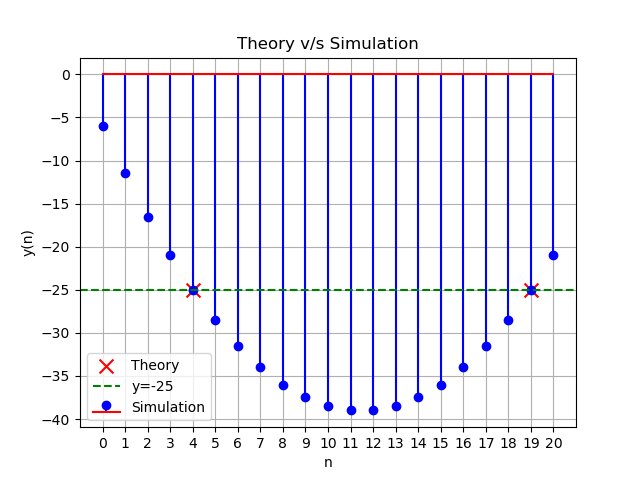
\includegraphics[width=1\linewidth]{figs/plot.png}
    \caption{Theory matches with simulated values}
    \label{fig:enter-label}
\end{figure}
\end{document}
